%%%%%%%%%%%%%%%%%%%%%%%%%%%%%%%%%%%%%%%%%%%%%%%%%%%%%%%%%%%%%%%%%%%%%%%%%%%%
%% Trim Size: 9.75in x 6.5in
%% Text Area: 8in (include Runningheads) x 5in
%% ws-ijprai.cls   :   8-8-2014
%% Class file to use with ws-ijprai.tex written in Latex2E.
%% The content, structure, format and layout of this style file is the
%% property of World Scientific Publishing Co. Pte. Ltd.
%% Copyright 2014 by World Scientific Publishing Co.
%% All rights are reserved.
%%%%%%%%%%%%%%%%%%%%%%%%%%%%%%%%%%%%%%%%%%%%%%%%%%%%%%%%%%%%%%%%%%%%%%%%%%%%
%

\documentclass{ws-ijprai}
\usepackage{enumerate}
\begin{document}

\markboth{Zhan Peng et al.}{An Efficient Algorithm for Suffix Sorting}

%%%%%%%%%%%%%%%%%%%%% Publisher's area please ignore %%%%%%%%%%%%%%%
%
\catchline{}{}{}{}{}
%
%%%%%%%%%%%%%%%%%%%%%%%%%%%%%%%%%%%%%%%%%%%%%%%%%%%%%%%%%%%%%%%%%%%%

\title{An Efficient Algorithm for Suffix Sorting}


\author{Zhan Peng$^1$, Yuping Wang$^1$\footnote{Corresponding author}~,
Xingsi Xue$^2$, Jingxuan Wei$^1$}

\address{$^1$School of Computer Science and Technology\\
  Xidian University\\
  Xi'an, Shaanxi, 710071, China\\
   $^*$ywang@xidian.edu.cn
}

\address{$^2$School of Information Science and Engineering\\
  Fujian University of Technology\\
  Fuzhou, Fujian, 350118, China\\}

\maketitle

%begin{history}
%received{(Day Month Year)}
%revised{(Day Month Year)}
%accepted{(Day Month Year)}
%comby{(xxxxxxxxxx)}
%end{history}

\begin{abstract} The Suffix Array (SA) is a fundamental data structure
which is widely used in the applications such as string matching, text
index and computation biology, etc. How to sort the suffixes of a string in
lexicographical order is a primary problem in constructing SAs, and
one of the widely used suffix sorting algorithms is
\emph{qsufsort}. However, \emph{qsufsort} suffers one critical
limitation that the order of suffixes starting with the same $2^k$
characters can not be determined in the $k$-th round. To this point,
in our paper, an efficient suffix sorting algorithm called
\emph{dsufsort} is proposed by overcoming the drawback of the
\emph{qsufsort} algorithm. In particular, our proposal maintains the
\emph{depth} of each unsorted portion of SA, and sorts the suffixes
based on the \emph{depth} in each round. By this means, some suffixes
that can not be sorted by \emph{qsufsort} in each round can be sorted
now, as a result, more sorting results in current round can be
utilized by the latter rounds and the total number of sorting rounds
will be reduced, which means \emph{dsufsort} is more efficient than
\emph{qsufsort}. The experimental results shows the effectiveness of
the proposed algorithm, especially for the text with high repetitions.
\end{abstract}

\keywords{suffix sorting; suffix array; text index; computation
biology}

\chapter{一种高效的后缀排序算法}
\section{引言}
\label{sec:introduction}

如何将给定字符串的所有后缀按照字典序进行排序, 是构建后缀数组(SA)的主要
问题. 目前, \emph{qsufsort}\cite{qsufsort} 算法是解决该问题广泛使用的算
法之一. 该算法对后缀进行逐轮排序, 每一轮的排序将基于上一轮的结果, 直到
所有后缀都处于正确的字典序. 具体地, 首先所有后缀将根据其首字符进行排
序, 然后在每一轮中, 排序所依据的字符数将翻倍, 这样, 在第\emph{k}轮之
后, 所有后缀将根据其前 $2^{k}$ 个字符进行排序. 这也意味着, 对于那些
前$2^{k}$字符相同的后缀, 它们的次序无法在第$k$轮之后被确定. 因此, 对于
那些具有较大 \emph{LCP}(Length of the Longest Common Prefix)的后缀,
\emph{qsufsort} 需要许多轮才能确定它们的次序, 这会严重影响算法效率.

为了克服 \emph{qsufsort} 的这种缺陷, 在本章中, 将提出一种基
于 \emph{qsufsort} 算法的改进的后缀排序算法--\emph{dsufsort}. 其核心思
想在于, 对后缀数组SA中每一个还未排序的部分(称作一个''桶''(bucket)),
\emph{dsufsort} 算法将记录该桶中所包含后缀(已知的)最大的\emph{LCP} (称
为该桶的''深度''), 并且在运行过程中对其进行实时更新. 然后, 在每一轮中,
每一个未排序桶中的后缀, 将基于该桶的深度进行排序. 通过这种方式, 许多后
缀在第$k$轮中, 可以基于超过前$2^k$个字符进行排序. 这意味
着, 在第$k$轮中, 无法由\emph{qsufsort}算法确定顺序的那些前$2^{k}$字符相
同的后缀, 有可能在$k$轮中被确定顺序. 由于在每轮中有更多的后缀能够被排
序, 因此有更多的排序结果可以被后面的过程所利用, 这会减少总共所需要的轮
数. 因此, \emph{dsufsort} 比 \emph{qsufsort} 更加高效, 尤其对于拥有较
大 \emph{LCP} 的后缀.

本章内容组织如下: 第2节介绍相关工作. 第3节将给出所用的符号和术语.
\emph{qsufsort} 和改进的 \emph{dsufsort} 算法将在第4节中进行详细介
绍. 第5节将讨论一些高效的实现技术. 第6节进行实验对比. 第7节是对本章进行
总结.

\section{相关工作}

在过去的二十年中, 大量的具有不同时间和空间复杂度的后缀数组构建算法(即后
缀排序算法) 被提出. 接下来, 将对其中的一些算法进行简要地回顾, 对其更详
细的介绍, 可参考综述文献 \cite{survey1,survey2}.

从后缀树来构造后缀数组, 是构建后缀数组最简单的方法之一, 其主要缺陷在于
过高的空间和和时间开销. Manber 和 Myers\cite{Manber} 第一个提出了直接构
建后缀数组的算法, 其时间复杂度为 $O(nlog^n)$ (其中$n$是给定字符串的长
度). 该算法使用了一种被称为''前缀倍增''的技术(最早来源
于Karp\cite{Karp}): 首先, 后缀将按照其首字符进行排序, 接着在之后的每一
轮中, 将按照加倍长度的前缀对后缀进行排序.
Larsson和Sadakane\cite{qsufsort} 提出了 \emph{qsufsort} 算法对Manber的
算法进行改进. 与Manber算法在每一轮中都需要检查SA中所有的桶不同,
\emph{qsufsort} 算法会标记那些之前已经被排过序的桶. 这样, 在每轮中它将
跳过那些被标记的桶, 只对未排序的桶进行排序. 尽管在理论上,
\emph{qsufsort} 算法和Manber的算法具有相同的时间复杂度, 在实际当中,
\emph{qsufsort}算法要高效得多. Schurmann\cite{bpr} 提出了一种具
有 $O(n^2)$ 时间复杂度的方法-- \emph{bpr}. 与Manber算法
和 \emph{qsufsort} 算法在每一轮中使用广度优先策略来对每一个桶进行排序不
同, \emph{bpr} 使用了深度优先的排序策略: 对于每一个未排序的桶, 它将递归
地对其中的后缀进行排序, 直到所有后缀都被完全排序.  Rajasekaran
\cite{RadixSA} 提出了被称为 \emph{RadixSA} 的新算法, 该算法具
有 $O(nlog^n)$ 的时间复杂度. 与前面三个算法使用简单的从左到右的顺序来对
桶进行排序不同, \emph{RadixSA} 使用了特殊的排序顺序: 假设第$i$个后
缀 $S_i$ 处于桶$B_i$中, 那么算法将首先对桶 $B_n$ 进行排序, 然后依次对
桶 $B_{n-1},\,\dots,\, B_1$ 进行排序. 这种顺序确保了在对桶 $B_i$ 排序之
后, 后缀$S_i$ 已经处于其在SA中的最终位置.

Seward\cite{Copy_Cache} 提出了另外两个后缀排序算法:
\emph{Copy} 和 \emph{Cache}. 它们首先将基于后缀的前两个字符对其进行排
序, 然后按照由小到大的顺序(即根据桶中所包含后缀的多少,由少到多)对未排
序的桶进行排序, 一旦一个桶被完全排好序, 排序的结果将被后续过程使用. 然
而, \emph{Copy} 和 \emph{Cache} 使用相同的函数对所有后缀进行排序, 这对
具有很长公共前缀的后缀(即具有较大$LCP$的后缀)效率不高. 为解决此问题,
Manzini\cite{deep_shallow} 提出了被称为 \emph{deep-shallow} 的算法. 当
对一个桶进行排序时, \emph{deep-shallow} 会使用\emph{shallow} 排序函数对
具有较短公共前缀的后缀进行排序, 而使用 \emph{deep} 排序函数对具有较长
公共前缀的后缀进行排序。 尽管 \emph{deep-shallow} 在理论上有良好的性能,但
复杂的框架限制了它在实际当中的使用。

以上所介绍的算法都具有超线性的时间复杂度。 然而, 已经有线性时间复杂度的
算法被提出,比较知名的包括 \emph{KA}\cite{KA},
\emph{KS}\cite{KS} 和 \emph{KSP}\cite{KSP} 算法. \emph{KSP} 算法采用了
和Farach算法\cite{Farach} 类似地归并策略。 \emph{KS} 算法使用了分而治之
的策略,包含3步: (1) 递归地为那些起始于位置 $i$ ($i~mod~3 \neq 0$) 的后
缀构造后缀数组; (2) 使用第一步的排序结果,为那些剩余后缀构建后缀数
组; (3) 将第一步和第二步中构建的后缀数组合并为一个. \emph{KA} 算法
是 \emph{two-stage} 算法\cite{two_stages} 的一个改进, 它将字符串中的所
有后缀分成两类:L-类和S-类。 然后递归地对所有L-类后缀进行排序,之
后,S-类后缀的顺序可由L-类后缀的顺序诱导得到。 Nong\cite{SA_IS_DS}提出
了两个算法 \emph{SA-IS} 和 \emph{SA-DS} 来改进 \emph{KA} 算法。 它们分
别使用了“变长最左S-类子串”和“定长d-关键子串”来对问题进行规约, 同时
使用了简单高效的算法对这些采样子串进行排序。 最近, Nong\cite{SACA_K} 针
对常量字符集又提出了一个线性时间算法--\emph{SACA-K}, 该算法仅需
要 $O(1)$ 大小的工作空间. 尽管线性时间算法在理论上具有较好的时间复杂度,
但在实际应用中, 它们的性能却常常不如在实现方面经过高度优化过的超线性算
法\cite{RadixSA}.

目前, 有许多外存算法\cite{em_1,em_2,em_3} 被提出用于构建较大的后缀数组,外
存算法所需要的空间主要由价格低廉且空间巨大的磁盘来提供。 通过使用外存算
法,可以构造出那些无法放入内存的巨大后缀数组。

\section{相关概念}
\label{sec:stucture}

令 $\Sigma$ 表示有限个字符组成的字符集 (本章只关注于ASCII字符
集, 即 $|\Sigma| = 256$ 且每个字符占用一个字节的存储空间.)  给定字符
$\Sigma$ can be defined as:\\

\textbf{定义 1.} $\Sigma$ 上的字符串是由有限个 $\Sigma$ 中的字符组成的
序列. $\Sigma$ 上长为$n$的字符串可表示为: $T =
t_0t_1..t_{n-1}$, 其中 $T[i] = t_i \in \Sigma$ $(0 \leq i \leq
n-1)$. A substring of $T$ is a sequence consisting of any consecutive
characters of $T$. $S$ 的一个子串是由 $s$ 中任意个连续字符所构成的字符
串. $T$中, 起始于位置 $i$ 且终止于位置 $j$ 的子串可表示 $T[i,j]$.\\
\\
在后缀排序中,最基本的概念是后缀和前缀,它们都是给定字符串特殊的子串,
定义如下:\\
\\
\textbf{定义2.} 对于字符串 $T = t_0t_1..t_{n-1}$, 其起始于位置
$i(0 \leq i \leq n-1)$ 的后缀是子串 $T[i,n-1]$, 由$S_i(T)$表示.  $T$ 的
长为 $h$ 的前缀是子串 $T[0,h-1]$, 由 $P_h(T)$ 表示.\\
\\
在本章中, 当提及某些后缀时, 它们一定是关联于同一个字符串的,所以符
号 $S_i(T)$ 可以无歧义地简写成 $S_i$. 为了确保没有后缀是其它某个后缀的
前缀, 通常会向字符串 $T$ 的末尾插入一个特殊字符 '\$', '\$' 被定义为在
字典序上小于任何 $\Sigma$ 中的字符.\\
\\
使用表达式 $S_i \prec S_j$ 来表示后缀 $S_i$ 以字典序小于后缀 $S_j$. 且
我们的最终目标是, 将给定字符串的所有后缀按照字典序由小到大进行排序, 形
成后缀数组:\\
\\
\textbf{定义 3.} 给定字符串 $T = t_0t_1..t_{n-1}\$$, $T$ 的后缀数
组(SA)是一个具有 $n+1$ 个元素的数组 $SA[0 \dots n]$, 其元素是 $0 \sim
n$ 的整数, 使得对于任意 $0
\leq i < j \leq n$, 都有 $S_{SA[i]} \prec S_{SA[j]}$.\\
\\
由于一个后缀可以唯一地由其起始位置确定, 只需要在SA中存储后缀的起始位置.\\
\\
为了简单起见, 术语"(后缀的)顺序"如果不做特殊说明, 将总是代表字典序. 基
于字典序, 可以通过只比较后缀的前$h$个字符, 来进一步定义后缀
的 \emph{h-序}: $S_i$ 被称为 \emph{h-小于} $S_j$ 当且仅当 $P_h(S_i)
\prec P_h(S_j)$, 这种关系被表示为 $S_i \prec_h S_j$.  同理, 符号
$=_h$ 和 $\preceq_h$ 可以被类似地定义. 明显地, 有: $S_i \prec_h S_j
\Longrightarrow S_i \prec S_j$. 如果所有的后缀都都依据其前
$h$ 个字符被排好序, 则它们被称为是\emph{h-有序}的.\\
\\
接下来将介绍"桶"(bucket)的概
念, 它是 \emph{qsufsort} 和 \emph{dsufsort} 算法中的核心概念.\\
\\
\textbf{定义 4.} 给定后缀数组SA, SA上一个深度为$h$的桶, 是一个子数
组 $SA[l \dots r]$ $(l \leq r)$ 满足: $S_{SA[l]} =_h S_{SA[l+1]}\dots
=_h S_{SA[r]}$ 且 $S_{SA[l-1]} \neq_h S_{SA[l]}$ 及 $S_{SA[r]} \neq_h
S_{SA[r+1]}$. 桶 $SA[l \dots r]$ 的序号被定义为 $l$, 该桶被表示
为 $B_l$.\\
\\
注意, 深度 \emph{h} 是桶
$B_l$ 中所包含后缀\emph{当前已知的}公共前缀的长度. 为了记录每一个后缀所
在的桶, 使用一个数组 $B$: 若 $B[i] = j$, 则 $S_i$ 当前处于
桶 $B_j$ 中. 注意区别: $B_i$ 是编号为 $i$ 的桶, 而 $B[i]$ 是后缀
$S_i$ 当前所在桶的编号.\\
\\
给定后缀 $S_i$ 和 $S_j$, $LCP(S_i, S_j)$ 被定义为 $S_i$ 和
$S_j$ 最长公共前缀的长度. 基于 $LCP(S_i,
S_j)$, 字符串的平均 \emph{LCP} 可以按如下定义:\\
\\
给定长为$n+1$的字符串 $T$ 及其后缀数组 $SA$, $T$
的平均$LCP$由以下公式计算:\\

\begin{equation}
\frac{1}{n}\sum_{i=0}^{n-1}LCP(S_{SA[i]},S_{SA[i+1]}).
\end{equation}

字符串的平均$LCP$, 可以粗略地估计对该字符串后缀进行排序所需的计算量: 如
果平均$LCP$较大, 原则上我们将需要比较更多的字符来确定两个后缀的顺序.

\section{ \emph{dsufsort} 算法}

本节将介绍基于 \emph{qsufsort} 算法的改进的后缀排序算法--
\emph{dsufsort}. \emph{dsufsort} 通过在排序过程中实时地维护每个桶的深度
来提高 \emph{qsufsort} 算法的效率. 当对某个桶进行处理时, 将根据桶的深度
对其中的后缀进行排序. 通过这种方式, 相比 \emph{qsufsort} 算法,
\emph{dsufsort} 算法在每一轮中可以确定更多后缀的顺序, 换言之, 对所有后
缀进行排序, \emph{dsufsort} 算法将需要较少的轮数, 这能够减少算法的运行
时间, 提高算法效率. 接下来, 先简要地介绍 \emph{qsufsort} 算法的核心思
想, 然后详细地讨论对其的改进算法 \emph{dsufsort}.

\subsection{ \emph{qsufsort}算法简介}
\label{sec:qsufsort}

Larsson和Sadakane所提出的 \emph{qsufsort} 算法使用了被称为''前缀倍
增''的技术来对后缀进行逐轮排序. 在第0轮中, 给定字符串的所有后缀将根据其
首字符进行排序. 之后, 所有具有相同首字符的后缀都会被排列到一起形
成$SA$上一个深度为1的桶, 而整个 $SA$ 将(在逻辑上)被划分为一系列的深度
为1的桶: 第一个桶中所包含的后缀具有最小的字符, 第二个桶中所包含的后缀具
有次小的字符, .... 依此类推.

注意, 如果一个深度为1的桶只包含一个后缀, 该桶及其包含的单个后缀被称为
是\emph{完全排序的}. 由于该后缀可以由其首字符从其它后缀中区分出来, 它已
经处于SA的最终位置, 将来无需再对其进行排序. 然而, 如果一个深度为1的桶包
含了超过一个后缀, 该桶及其所包含的后缀则被称为是\emph{未排序的}, 在未
来, 将需要比较更多的字符来确定其后缀的顺序.

在第0轮后, 所有后缀都处于\emph{1-有序}的状态. 并且不失一般性地, 任意两
个后缀 $S_i$ 和 $S_j$ 的1-序可由其所在桶的序号确定:
$S_i \preceq_1 S_j \iff B[i] \leq B[j]$.

通过使用前缀倍增技术, 在每轮过后, 所有的后缀都将基于其倍增长度的前缀被
排序. 这样, 在第 \emph{k-1} 轮之后, 所有的后缀都将处于 $2^{k-1}$-有序,
换言之, 所有未排序的桶都有同样的深度 $2^{k-1}$, 且这些未排序的桶, 将在
第$k$轮中被从左到右逐个进行排序.

Now, assuming an unsorted bucket $B_p$ is being sorted in the $k$-th
round. For any $S_i$ and $S_j$ in $B_p$, since $S_i =_{2^{k-1}} S_j$,
the order of $S_i$ and $S_j$ will depend on the order of
$S_{i+2^{k-1}}$ and $S_{j+2^{k-1}}$, that is $S_i \prec S_j \iff
S_{i+2^{k-1}} \prec S_{j+2^{k-1}}$, without loss of generality. Here,
$S_{i+2^{k-1}}$($S_{j+2^{k-1}}$) is called the \emph{anchor suffix} of
$S_i$($S_j$). However, since only the $2^{k-1}$-order of
$S_{i+2^{k-1}}$ and $S_{j+2^{k-1}}$ is known now, only the $2^k$-order
of $S_i$ and $S_j$ can be determined: $S_i \preceq_{2^k} S_j \iff
S_{i+2^{k-1}} \preceq_{2^{k-1}} S_{j+2^{k-1}} \iff B[i+2^{k-1}] \leq
B[j+2^{k-1}]$.  This derivation gives a way to sort the suffixes of
$B_p$ in $2^k$-order: for any $S_i$ in the $B_p$, the value
$B[i+2^{k-1}]$, which is the bucket number of $S_i$'s anchor suffix,
can be used as the \emph{key} of $S_i$ :$key(S_i) = B[i+2^{k-1}]$, and
then all the keys of the suffixes are sorted first by a common integer
sorting routine, after that the suffixes in the $B_p$ can be sorted in
$2^k$-order by being simply rearranged according to the arithmetic
order of their keys.

Once an unsorted bucket is sorted, new buckets are formed according to
the following two cases: 1) If a suffix has a unique key, it will be
in its final location in SA to form a singleton bucket which is
completely sorted. 2) If some suffixes have the same key, they will be
rearranged together and form a new unsorted bucket which will be
sorted in future rounds. And the $B$ array needs to be updated
according to these new buckets.

The \emph{qsufsort} algorithm runs round by round untill there is no
unsorted bucket left. Note that, using the prefix doubling technique,
the length of the checked prefix of each suffix is doubled after each
round, so for any two suffixes of the input string, their order can
be determined in at most $log^n$ rounds, where $n$ is the length of
the input string. Therefore the \emph{qsufsort} algorithm performs up
to $log^n$ rounds to completely sort all the suffixes.

\subsection{The dsufsort algorithm: maintaining the depth for
each unsorted bucket}
\label{sec:dsufsort}

As stated above, in the $k$-th round, the \emph{qsufsort} algorithm
checks only the first $2^k$ characters of each suffix to determine
their order, which means the order of the suffixes starting with the same
$2^k$ characters can not be determined in the $k$-th round. Therefore
for suffixes with a long common prefix, \emph{qsufsort} needs several
rounds to determine their order, which will lead to a great
computation cost.

It is necessary to reduce the computation cost by checking as many
characters of each suffix as possible to determine their order in each
round. To achieve this purpose, for each unsorted bucket, the
\emph{dsufsort} algorithm maintains its \emph{bucket depth} (length of
the common prefix of its suffixes that we have currently know), and
updates the bucket depth once an unsorted bucket is sorted. In each
round, when sorting the suffixes in an unsorted bucket, the
\emph{dsufsort} uses the depth of the bucket to compute the keys of
the suffixes and then sort them.  Using the keys which are computed
from the bucket depth, the suffixes of some unsorted buckets can be
sorted according to more than the most-left $2^k$ characters in the
$k$-th round, as a result, some of the suffixes starting with the same
$2^k$ characters can be completely sorted by \emph{dsufsort} in the
$k$-round. Therefore the \emph{dsufsort} can sort more suffixes than
the \emph{qsufsort} in each round, and it usually uses fewer sorting
rounds.

In order to store the depth information, an array $D$ is created.
The depth of a bucket can be indexed by its bucket number: for a
bucket $B_p$, its depth is recorded in $D[p]$. After round 0, we set
$D[p] = 1$ for each unsorted bucket $B_p$.

Similar to \emph{qsufsort}, the \emph{dsufsort} algorithm works round
by round until there is no unsorted bucket left. In each round, the
\emph{dsufsort} algorithm adopts a two phases \emph{sorting --
updating} strategy to sort each unsorted bucket and update their
depths. As an example, suppose an unsorted bucket $B_p$ is being
sorted in the $k$-th round.

\begin{arabiclist}
\item \textbf{Sorting:} for any $S_i$ and $S_j$ in $B_p$, since $S_i
=_{D[p]} S_j$, the order of $S_i$ and $S_j$ is depend on the order of
$S_{i+D[p]}$ and $S_{j+D[p]}$: $S_i \prec S_j \iff S_{i+D[p]} \prec
S_{j+D[p]} \iff B[i+D[p]] < B[j+D[p]]$, without loss of
generality. Here $S_{i+D[p]}$($S_{j+D[p]}$) is the \emph{anchor
suffix} of $S_i$($S_j$). According to this relation, for any $S_i$ in
$B_p$, the \emph{dsufsort} algorithm takes $B[i+D[p]]$ (rather than
$B[i+2^{k-1}]$ which is used in \emph{qsufsort}) as its key, and then
sort the keys of suffixes with a common integer sorting
algorithm. After that, the suffixes in $B_p$ are rearranged according
to their keys.

After rearranging, for each suffix $S_i$ in $B_p$, it is sorted according to the first
$D[p] + D[B[i+D[p]]$ rather than $2^k$ characters.  We will soon see
that in the $k$-th round(after the (\emph{k-1})-th round), there must
be $D[p] \geq 2^{k-1}$ and $D[B[i+D[p]] \geq 2^{k-1}$, which means the
suffixes are sorted according to \emph{at least} the first $2^k$
characters, thus the \emph{dsufsort} can perform at least as good as
\emph{qsufsort}. And we will also see that in some case, there holds
$D[p] > 2^{k-1}$, which means all the suffixes in $B_p$ are sorted
according to more than $2^k$ characters, and in this case the
\emph{dsufsort} algorithm performs better than \emph{qsufsort}.

\item \textbf{Updating:} the $D$ and $B$ array will be updated immediately
once $B_p$ is sorted. Suppose the suffixes are rearranged as $S_{i_1},
S_{i_2},\dots,S_{i_s}$ according to their keys $key(S_{i_1}) \leq
key(S_{i_2}) \leq \dots \leq key(S_{i_s})$. Depending on whether or
not the key of a suffix is unique, there are two kinds of suffixes:

\begin{itemize}

\item For any $S_{i_j}$ such that $key(S_{i_{j-1}}) \neq key(S_{i_j})$
and $key(S_{i_j}) \neq key(S_{i_{j+1}})$, $S_{i_j}$ will be in its
final location in SA and forms a completely sorted singleton bucket:
$B_{p+j-1}$. The bucket of $S_{i_j}$ is updated accordingly: $B[i_j]$
is updated to $p+j-1$. However, there is no need to update the depth
(the $D$ array) for completely sorted buckets.

\item For each group of suffixes $\{S_{i_l},
S_{i_{l+1}},\dots,S_{i_r}\}$ such that: $key(S_{i_l}) =
key(S_{i_{l+1}}) = \dots = key(S_{i_r}) = m$, $key(S_{i_{l-1}}) \neq
m$ and $key(S_{i_{r+1}}) \neq m$, the group $\{S_{i_l},
S_{i_{l+1}},\dots,S_{i_r}\}$ will form a new unsorted bucket :
$B_{p+l-1}$. Since every suffix in $B_{p+l-1}$ has its anchor suffix
in $B_m$, $B_m$ is called the \emph{anchor bucket} of $B_{p+l-1}$. The
bucket of each suffix in the group is updated accordingly: all of
$B[i_l], B[i_{l+1}], \dots, B[i_r]$ are updated to $p+l-1$.  Since we
have already known that $S_{i_l} =_{D[p]} S_{i_{l+1}} =_{D[p]} \dots
=_{D[p]} S_{i_r}$ and $S_{i_l+D[p]} =_{D[m]} S_{i_{l+1}+D[p]} =_{D[m]}
\dots =_{D[m]} S_{r+D[p]}$, there holds $S_{i_l} =_{D[p]+D[m]}
S_{i_{l+1}} =_{D[p]+D[m]} \dots =_{D[p]+D[m]} S_{i_r}$.  Therefore the
depth of the newly created bucket $B_{p+l-1}$ is: $D[p+l-1] = D[p] +
D[m]$, and we will use this formula to update the depth for each newly
created unsorted bucket.
\end{itemize}
\end{arabiclist}


Based on the two phases \emph{sorting -- updating} strategy, the
framework of \emph{dsufsort} can be summarized bellow:

\begin{enumerate}[\hspace{0.3cm} \bfseries Step 1.]

\item Initialization(round 0): sort all the suffixes of a given
string according to their first characters. For each unsorted bucket
$B_p$, set $D[p] = 1$, and for any $S_i$ in $B_p$, set $B[i] = p$.

\item For each unsorted bucket (say $B_p$) left in
SA, perform the following \emph{sorting -- updating} procedure:

\begin{enumerate}[\bfseries i.]
\item \emph{Sorting}: for each suffix $S_i$ in $B_p$, taking
$B[i+D[p]]$ as its key, and sort the keys of suffixes by an integer
sorting algorithm. Rearrange the suffixes in $B_p$ according to the
arithmetic order of their keys.
\item \emph{Updating}: suppose the suffixes in $B_p$ are rearranged
as: $S_{i_1}, S_{i_2},\dots,S_{i_s}$. For any $S_{i_j}$ such that:
$key(S_{i_{j-1}}) \neq key(S_{i_j})$ and $key(S_{i_j}) \neq
key(S_{i_{j+1}})$, set $B[i_j]$ to $p+j-1$. For each group of suffixes
$\{S_{i_l}, S_{i_{l+1}},\dots,S_{i_r}\}$ such that $key(S_{i_l}) =
key(S_{i_{l+1}}) = \dots = key(S_{i_r}) = m$, $key(S_{i_{l-1}}) \neq
m$ and $key(S_{i_{r+1}}) \neq m$, create a new unsorted bucket
$B_{p+l-1}$for that group.  Set $D[p+l-1]$ to $D[p] + D[m]$, and set
all of $B[i_l], B[i_{l+1}], \dots, B[i_r]$ to $p+l-1$.
\end{enumerate}

\item If there are no unsorted buckets left in $SA$, stop and quit;
otherwise, go to step 2 and start a new sorting round.

\end{enumerate}

As stated before, the \emph{dsufsort} algorithm has the following important feature:

\begin{lemma}
  For any unsorted bucket $B_q$ created in the k-th round \emph{(}$k =
0,1,2,\dots$ \emph{)}, there holds: $D[q] \geq 2^k$.
\end{lemma}

\begin{proof} This can be proved by induction. Basis: for any unsorted
bucket $B_q$ created in round 0, there holds $D[q] = 1 \geq 2^0$.
Induction: suppose $B_q$ is an unsorted bucket created from $B_p$ in
the $k$-th round, and $B_m$ is the anchor bucket of $B_q$. Since $B_p$
and $B_m$ are unsorted buckets created in the (\emph{k-1})-th round,
by induction, there holds $D[p] \geq 2^{k-1}$ and $D[m] \geq 2^{k-1}$
, therefore $D[q] = D[p] + D[m] \geq 2^{k-1} + 2^{k-1} = 2^k$.
\end{proof}

This feature ensures that the
\emph{dsufsort} algorithm can perform at least as good as
\emph{qsufsort}. However it is necessary to explore in which case the
\emph{dsufsort} performs better, specially, in which
case there is $D[q] > 2^k$. Suppose we are in the (\emph{k-1})-th
round, and sort an unsorted bucket $B_p$ which is created in the
(\emph{k-2})-th round with $D[p] = 2^{k-2}$. If a new unsorted
bucket $B_q$ is created from $B_p$ and its anchor bucket is $B_m$,
there is $D[q] = D[p] + D[m]$.

The key point is that, if $B_m$, which is the anchor bucket of $B_p$,
is also a new unsorted bucket that created previously in the
(\emph{k-1})-th round, due to the feature we have just proved, there
must be $D[m] \geq 2^{k-1}$. So we have $D[q] = D[p] + D[m] \geq
2^{k-2} + 2^{k-1} > 2^{k-1}$, which means the depth of $B_q$ is
strictly larger than $2^{k-1}$. Consequently, when $B_q$ is processed
in the \emph{k}-th round, any $S_i$ in $B_p$ is sorted according to
its first $D[p] + D[B[i+D[p]]$ characters as stated before, since
$D[q] > 2^{k-1}$ and $D[B[i+D[p]] \geq 2^{k-1}$, $S_i$ is sorted
according to more than $2^k$ characters in the $k$-th round, which
means the \emph{dsufsort} algorithm performs better than \emph{qsufsort}. Furthermore, if
$B_m$ is in the same case as $B_q$, that is, the anchor bucket of
$B_m$ is also a bucket created in the (\emph{k-1})-round, then there
is $D[m] > 2^{k-1}$. Due to the \emph{accumulation of the depths},
$D[q]$ can be much larger than $2^{k-1}$, as a result, the suffixes in
$B_q$ can be sorted according to much more than $2^k$ characters in
the $k$-th round.

\begin{figure}[bh]
\centerline{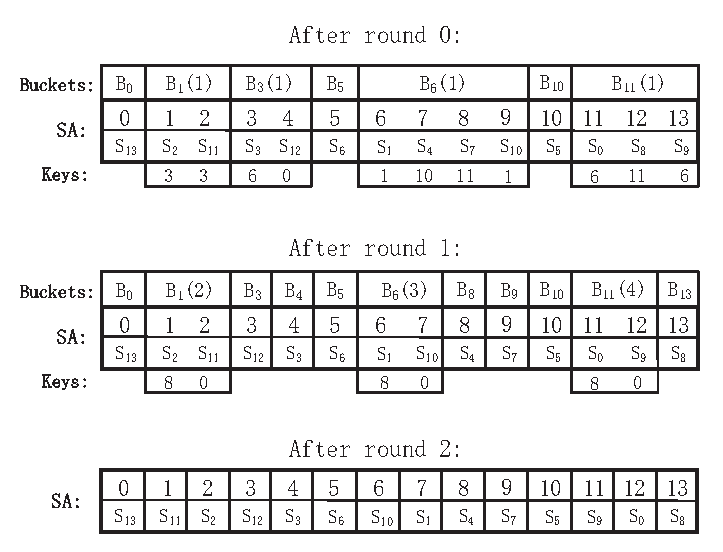
\includegraphics[width=9cm]{p1}}
\vspace*{8pt}
\caption{An example run of the \emph{dsufsort} algorithm with the input
    string '\emph{tobeornottobe}'.}
\label{fig:1}
\end{figure}

\textbf{Example.} Figure \ref{fig:1} shows the procedure of the
\emph{dsufsort} algorithm with the input string
'\emph{tobeornottobe}'. For clearly show, we put $S_i$ in SA instead
of its starting position $i$. The depth of a bucket is shown in the
parentheses following the bucket. After round 0, all the suffixes are
sorted according to their first characters. Since each of $B_0$, $B_5$
and $B_{10}$ contains a single suffix, these three buckets are completely sorted.

In round 1, the four unsorted buckets $B_1$, $B_3$, $B_6$ and $B_{11}$
left from round 0 are sorted in order. As an example, we sort $B_6$,
and the other three buckets can be sorted in the same way. For any
$S_i$ in $B_6$, its key can be computed from the bucket depth by
$key(S_i) = B[i+D[6]]$. So the keys of suffixes of $B_6$ are:
$key(S_1) = B[1+D[6]] = 1$, $key(S_4) = B[4+D[6]] = 10$, $key(S_7) =
B[7+D[6]] = 11$, $key(S_{10}) = B[10+D[6]] = 1$. Then these keys are
sorted by a regular integer sorting algorithm to have the order: $key(S_1) = key(S_{10})
< key(S_4) < key(S_7)$.  According to the arithmetic order of their
keys, the 1-order of the suffixes in $B_6$ can be determined: $S_1 =_
1 S_{10} \prec_1 S_4 \prec_1 S_7$, and the suffixes are rearranged
accordingly. Since $S_1$ and $S_{10}$ have the same key, they will be
grouped together in a newly created unsorted bucket $B_6$. Note that,
compared with the \emph{old} $B_6$(denoted by $B_6^{\;old}$) which is
being processed now, the newly created $B_6$(denoted by $B_6^{\;new}$)
has the same bucket number (which means the bucket numbers of $S_1$ and
$S_{10}$ need not to be updated), but different size and depth. The
depth of $B_6^{\;new}$ is $D[6]^{\;new} = D[6]^{\;old} + D[1] = 3$,
because $B_1$ is the anchor bucket of $B_6^{\;new}$ and $D[1] = 2$.
On the other hand, $S_4$ and $S_7$, each of which has a unique key,
will be in completely sorted buckets $B_8$ and $B_9$ respectively, and
only get their bucket number updated: $B[4] = 8$, $B[7] = 9$.  After
round 1, there left three unsorted buckets: $B_1^{\;new}$,
$B_6^{\;new}$, $B_{11}^{\;new}$.

 In round 2, $B_1^{\;new}$, $B_6^{\;new}$ and $B_{11}^{\;new}$ will be
sorted in order. Using $D[1] = 2$, $D[6] = 3$, and $D[11] = 4$
respectively to compute the keys of suffixes and sort them in the
corresponding unsorted buckets, all these three buckets will be
completely sorted in this round, which ends the whole algorithm.

To illustrate the advantage of \emph{dsufsort} over \emph{qsufsort},
we examine the sorting process of $B_{11}^{\;old}$ in round 1 . Since
the keys of the suffixes in $B_{11}^{\;old}$ are: $key(S_0)=6$,
$key(S_9)=6$ and $key(S_8) = 11$, $S_8$ is completed sorted in
$B_{13}$, while $S_0$ and $S_9$ will be in unsorted bucket
$B_{11}^{\;new}$.  Since $B_{11}^{\;new}$ is created from
$B_{11}^{\;old}$, and its anchor bucket is $B_6^{\;new}$, the depth of
$B_{11}^{\;new}$ is $D[11]^{\;new} = D[11]^{\;old} + D[6]^{\;new}$. As
we have seen, $B_6^{\;new}$ is also created in round 1 with
$D[6]^{\;new} = 3$, so $D[11]^{\;new} = 1 + 3 = 4$. Therefore the
depth of $B_{11}^{\;new}$ is larger than 2 which is the ``depth'' of
all buckets computed by \emph{qsufsort} in round 1.  Consequently in
round 2, the suffixes contained in $B_{11}^{\;new}$ are sorted
according to at least their first $4 +2$ characters instead of $2 + 2
$ characters as in the \emph{qsufsort}. The keys of suffixes are:
$key(S_0)=B[0+D[11] ^{\;new}]= 8$ and $key(S_9)=B[9+D[11]^{\;new}]=
13$, which means $B_{11}$ can be completely sorted in round 2. By
contrast, in the \emph{qsufsort}, the keys of suffixes in
$B_{11}^{\;old}$ are $key(S_0) = B[0+2] = 1$ and $key(S_9) = B[9+2] =
1$ which means $B_{11}^{\;old}$ can not be completely sorted after the
second round.  The result is that \emph{dsufsort} algorithm only needs
3 rounds to completely sort all the suffixes, while \emph{qsufsort}
needs 4.

For the input string with a large \emph{average LCP}, the feature of
the \emph{depth accumulations} of \emph{dsufsort} can be fully used,
and the order of the suffixes with very long common prefix can be
determined much faster.


\section{Efficient Implementation}

In this section, we describe some techniques used to derive efficient
implementation of the proposed algorithm.

\subsection{Input transformation}

In round 0, the suffixes are sorted only according to their first
characters. Actually, they can be sorted according to the first
\emph{few} characters by using a technique called \emph{input
transformation} to the input string in advance. The \emph{input
transformation} includes the following  two phases:

\subsubsection{Alphabet compaction}

Given a text string $T = t_0t_1...t_{n-1}\$$ over $\Sigma$, suppose
the characters that actually appear in $T$ form an ordered set $C =
\{c_0, c_1,\dots, c_{m-1}\}$, in which $c_i < c_j \iff i < j$. Note
that, the smallest terminal character '\$' must be $c_0$.  Then, for
each character in $T$, we can replace that character by its
corresponding ordinal number in $C$, that is: $t_i \mapsto j \iff t_i
= c_j$.  By using this mapping, each character of $T$ is encoded as an
integer, and the order of suffixes is preserved. With the alphabet
compaction, $\Sigma$ is transformed into a smaller integer alphabet:
$\{0,1,\dots,m-1\}$.

\subsubsection{Characters aggregation}

After applying the alphabet compaction to $T$, we get a new alphabet
of size $m$: $\{0,1,\dots,m-1\}$. Let $k$ be the largest integer such
that $m^k-1$ can be held in a typical machine integer. Then, for each
suffix of $T$, we can aggregate its first $k$ characters into one
using the following formula:

\begin{equation}\label{eq:ca1}
  T[i] = \sum_{j=1}^k t_{i+j-1} \cdot m^{k-j}  ~~(0 \leq i \leq n),
\end{equation}

\noindent where we define $t_s = 0$, for $s \geq n$.  In round 0,
$T[i]$ is used as the key for $S_i$, thus, sorting is based on not
only the first character of each suffixes, but also the first $k$
characters. The subsequent rounds of sorting can start with bucket
depth $k$ instead of 1, and the number of rounds will be
reduced. Formula (\ref{eq:ca1}) can be computed in linear time through
an alternate form:

\begin{equation}\label{eq:ca2}
 T[i]  = \left\{
  \begin{array}{lll}
    \sum_{j=1}^{k}(t_{j-1} \cdot m^{k-j})  &,  &  i = 0\\
    (T[i-1]~ mod~m^{k-1}) \cdot m + t_{i-1+k} &,  & 0 < i \leq n \\
    \end{array}\right.
\end{equation}

\par\noindent
where $t_s = 0$, for $s \geq n$. The multiplication and modulo
operation can be replaced by faster bitwise operations \emph{shift}
and \emph{and}.

Note that, since the alphabet of $T$ may not be consecutive after
characters aggregation, we need to use alphabet compaction again to
the new aggregated string $T$.

\subsection{Initial bucket sorting}

The round 0 (initialization) of the algorithm is quite independent
to the rest of the algorithm and is not required to use the same
sorting method as the following rounds. Since this step must process
all of the suffixes in a single round, a substantial improvement
can be gained by using a linear time bucket sorting algorithm
instead of a comparison-based algorithm that requires $O(nlog^n)$
time.

A reasonable improvement can be gained by combining bucket sorting
with input transformation as described above. Given a string $T =
t_0t_1 \dots t_{n-1}\$$, suppose the new alphabet after applying input
transformation to $T$ is $I = \{0,1,\dots,m-1\}$. For each integer $i$ in
$I$, its number of occurrences in $T$ is counted and an array $F$ of size $m$ is
used to record that number. In particular, if integer $i$ occurs
$j$ times in $T$, then $F[i] = j$, and based on this definition, there
is $\sum_{i=0}^{m-1} F[i] = n + 1$. To conclude, the round 0 of the
\emph{dsufsort} algorithm using bucket sorting includes the following four steps:

\begin{arabiclist}
\item Initialize $F$: $\forall i \in I$, set $F[i] = 0$.
\item Scan $T$ forwards to compute the occurrence frequency of
its symbols: for $i = 0,\dots,n$, increment $F[T[i]]$ by 1.
\item Traverse $F$ forwards, and sum adjacent elements so as
to form cumulative frequency counts: for $i = 1, \dots, m-1$, set
$F[i] = F[i] + F[i-1]$.
\item Scan $T$ backwards to put each of its suffix in the proper
bucket: for $i = n, n-1,\dots, 0$, decrement $F[T[i]]$ by 1, and set
$SA[F[T[i]]] = i$.
\end{arabiclist}

After round 0, SA is partitioned into $m$ (completely sorted or
unsorted) buckets , and all suffixes in an unsorted bucket start with
the same $k$ characters. In essence, the term \emph{bucket} in the
\emph{bucket sort} here is exactly the depth-$k$ bucket defined by
Definition 5 in the Preliminaries.

\subsection{Choosing an integer sorting subroutine}

Both of the \emph{qsufsort} and the \emph{dsufsort} algorithm need an
integer sorting subroutine to sort the keys, thus, this subsidiary
subroutine may have a great effect on the performance of the whole
algorithms. The sorting subroutine used in this paper is called
\emph{split-end partitioning} which is proposed by Bentley and
Mcllroy\cite{t_quciksort}. It is a variant of the well known
\emph{Quicksort}\cite{quicksort}, but uses a \emph{ternary-split
partition} strategy.

The classical \emph{Quicksort} which uses a \emph{binary-split
partition} strategy recursively partitions an array into \emph{two}
parts, one with smaller elements than a pivot element and one with
larger elements. Then the parts are processed recursively until the
whole array is sorted. The \emph{Quicksort} mixes the elements being
equal to the pivot into one or both of the parts depending on the
implementation. However, the \emph{split-end partitioning} algorithm
which uses a ternary-split partition strategy generates \emph{three}
parts: one with elements smaller than the pivot, one with elements
equal to the pivot, and one with elements larger than the pivot. The
smaller and larger parts are then processed recursively while the
equal part is remained, since its elements are already correctly
placed.

The implementation of \emph{split-end partitioning} in our algorithm
is based on Program 7 of Bentley and Mcllroy \cite{t_quciksort} with
one exception: for fast handling of small buckets, a variant of
selection sort which is non-recursive is used to sort buckets with
less than 7 elements.


\section{Experimental Results}

We compared the \emph{dsufsort} algorithm to three well known
algorithms, i.e. the original \emph{qsufsort}
algorithm\cite{qsufsort}, the \emph{DC32}\cite{DC32} algorithm, and
the \emph{KS} algorithm\cite{KS}.  Our \emph{dsufsort} algorithm is an
improvement of \emph{qsufsort} algorithm. The \emph{DC32} is the
\emph{difference-cover} algorithm with difference-cover modulo 32.
The \emph{KS} algorithm is one of the fastest suffixes sorting
algorithms of a worst-case linear time complexity. We evaluated the
performance of these algorithms for real world data and for
degenerated data: artificial strings with very high \emph{average
LCP}.

The experiments were performed on a notebook running Ubuntu
14.04-64bit operating system with the following configuration: Intel
Core i7-2630QM 2.00GHz processor, 8GB 1333Mhz DDR3 SDRAM, 500GB SATA
disk. All the programs were implemented in C/C++, and compiled by
\emph{gcc} 4.8.2 with flags``--O3''. To ensure the correctness of the
testing algorithms, all the sorting results are checked by a
\emph{suffix array checker} which is described in
Burkhardt\cite{DC32}.

\begin{table}[th]
\tbl{Data sets used in the experiment.}
{ \begin{tabular}{@{}ccrrrr@{}} \toprule
  Files & Description & Size(bytes) & $\|\Sigma\|$ & Average LCP & Max LCP \\ \colrule
 Proteins & Protein sequence & 66,804,271 & 24 & 33.46 & 6380\\
 XML & XML files & 294,724,056 & 97 & 44.91 & 1084 \\
 Pitches & MIDI pitch values & 55,832,855 & 133 & 262.00 & 25178\\
 Sources & C/Java source code & 210,866,607 & 230 & 371.80 & 307871\\
 DNA & DNA sequence & 403,927,746 & 16 & 2420.73 & 1378596\\
 English & English text & 2,210,395,553 & 235  &6675.35 & 987770\\ \botrule
  \end{tabular}}
  \label{tab:data}
\end{table}

The real world data set we used in the experiment is the \emph{Pizza
 Chili Corpus}\cite{dataset} which contains six kinds of data:
source code, pitch values, protein sequence, DNA sequence, English
text, and XML files. The characteristic of the data set is shown in
Table 1 which shows the size, the average and maximum LCP
lengthes for each file. The average/maximum LCP for a string is the
average/maximum ones for all pairs of adjacent suffixes in the suffix
array .The maximum LCP length is equivalent to the length of the
longest repeated substring. These values give a good estimate of the
repetitiveness of the data.

\begin{table}
  \tbl{Sorting times in seconds.}
  { \begin{tabular}{crrrrr} \toprule
   Files & Size   & dsufsort  & qsufsort & DC32  & KS\\   \colrule
    Proteins   & 100MB  & 25.34 &\textbf{24.11}    & 35.43 & 98.91\\
    XML        & 100MB  & 27.59 &\textbf{26.75}    & 49.54 & 67.39 \\
    Pitches    & 50MB   &\textbf{9.27 } & 10.52    & 12.42 & 32.83 \\
    Sources    & 100MB  &\textbf{23.81} & 25.64    & 33.03 & 83.03 \\
    DNA        & 100MB  &\textbf{26.02} & 28.90    & 38.15 & 85.44 \\
    English    & 100MB  &\textbf{41.72} & 44.35    & 48.20 & 97.12 \\
    \colrule
    aaa\dots    & 100MB  &\textbf{9.14}  & 10.65 & 73.32 & 11.87\\
    abab\dots   & 100MB  &\textbf{8.82}  & 11.55 & 30.23 & 9.56\\
    rand-5-rep  & 100MB   &\textbf{10.36} & 16.32 & 35.60 & 12.77 \\
    rand-10-rep & 100MB   &\textbf{16.73} & 24.28 & 33.57 & 17.53 \\
    rand-20-rep & 100MB   & 23.11 & 39.03 & 35.92  & \textbf{22.85} \\
    \botrule
  \end{tabular}}
  \label{tab:time}
\end{table}

Table 2 shows the mean sorting time of each testing algorithm based on
10 independent runs, in which the best run times among all compared
algorithms are shown in bold. We also use artificial repetitive files
to test the robustness of the testing algorithms. The first two files
contain solely the letter \emph{a} and the pair \emph{ab}
respectively, and the following three files that have the form
`\emph{rand-k-rep}' are generated by a single random \emph{seed}
string of length $k$ which is repeated until 100MB characters are
reached.

From the results, we can see that, for real world data, the
\emph{dsufsort} and the \emph{qsufsort} perform best, and the
\emph{dsufsort} performs better than \emph{qsufsort} on most real
world data. Only for Proteins and XML files which have very low
\emph{average LCP}, \emph{dsufsort} performs a little bit worse than
\emph{qsufsort}. The reason is that, compared with \emph{qsufsort},
the \emph{dsufsort} needs to read and update the $D$ array during the
processing, and these operations require additional random memory
accesses which will lead to additional cache misses. So the time cost
will be over the one we saved from the \emph{depth accumulation} which
is not very effective for strings with very low \emph{average LCP}.

For artificial data whose \emph{average LCP} is relatively high, the
\emph{dsufsort} can dramatically reduce the time for sorting suffixes
with long \emph{LCP}. The results in Table 2 also show that
\emph{dsufsort} dominates others except for \emph{KS} on one file
(rand-20-rep) where the liner time algorithm \emph{KS} is faster. This
is because the performance of linear time algorithm is not severely
affected by the characteristic of input data.  However the \emph{KS}
algorithm performs not well for ordinary data, and this limits its
application in practice.

In summary, we can draw the conclusion that \emph{dsufsort}
algorithm outperforms the others in most cases. Only for case with
very low \emph{average LCP}, \emph{dsufsort} algorithm does not
outperform \emph{qsufsort}, and for case with very high
\emph{average LCP}, it does not outperform \emph{KS} algorithm
sometimes.

\section{Conclusions and Future Work}

In this paper, an efficient suffixes sorting algorithm,
i.e. \emph{dsufsort}, is proposed, which is based on the framework of
\emph{qsufsort}. Unlike the \emph{qsufsort} sort suffixes according to
a fixed number of characters in each round, \emph{dsufsort} maintains
the depth for each unsorted bucket, and sort the bucket based its
depth, furthermore, the \emph{accumulation of depths} during
processing makes \emph{dsufsort} very efficient, especially for
strings with large \emph{average LCP}.

There are two problems left for further research: Firstly, in our
implementation, the unsorted buckets are simply processed one by one
from left to right. However, the order in which the buckets are
processed can have an effect on the performance of algorithm, so what
is the best order from which the buckets should be processed?
Secondly, the $D$ array used to record the depth information may be
very sparse, which leads to unnecessary excessive memory
consumption. How to compact the $D$ array to reduce the space
complexity?

\section*{Acknowledgements}

This work is supported by National Natural Science Foundation of China
(No.61203372, No.61472297 and No.U1404622).

\begin{thebibliography}{99}

\bibitem{Manber} U. Manber and G. Myers, ``Suffix arrays: A new method
for on-line string searches,'' {\it SIAM J: Comput.}, {\bf 22}(1993)
935--948.

\bibitem{Karp} Karp RM, Miller RE and Rosenberg AL, ``Rapid
identification of repeated patterns in strings, trees and arrays,''
{\it Proc. 4th Ann. Theory of Computing}. ACM Press, New York, 1972,
pp.~125--136.

\bibitem{survey1} S.J. Puglisi, W.F. Smyth and A.H. Turpin, ``A
Taxonomy of Suffix Array Construction Algorithms,'' {\it ACM Computing
Surveys.} {\bf 39}(2007) 1--31.

\bibitem{survey2} J. Dhaliwal, S.J. Puglisi and A. Turpin, ``Trends in
Suffix Sorting: A Survey of Low Memory Algorithms,'' {\it
Proc. 12nd. Australasian Computer Science Conference}, Darlinghurst,
Australia, 2012. pp. ~91--98.

\bibitem{Copy_Cache} J. Seward, ``On the performance of BWT sorting
algorithms,'' {\it In DCC: Data Compression Conference}, IEEE Computer
Society Press, Los Alamitos, CA, 2000.  pp.~173--182

\bibitem{deep_shallow} Giovanni Manzini and Palol Ferragina,
``Engineering a lightweight suffix array construction
algorithm''. {\it Algorithmica}. {\bf 40}(2004) 33--50.

\bibitem{qsufsort} N. Larsson and K. Sadakane, ``Faster suffix
sorting,'' {\it Theor. Comput. Sci.} {\bf 387}(2007) 258--272.

\bibitem{bpr} K.-B. Schurmann and J. Stoye, ``An incomplex algorithm
for fast suffix array construction,'' {\it Softw. Pract. Exp.}  {\bf
37}(2007) 309--329.

\bibitem{RadixSA} S. Rajasekaran and M. Nicolae, ``An elegant
algorithm for the construction of suffix arrays,'' {\it J.  Discrete
Algorithms}. {\bf 27} (2014) 21--28.

\bibitem{KA} P. Ko and S. Aluru, ``Space Efficient Linear Time
Construction of Suffix Arrays,'' {\it J. Discrete Algoritms.} {\bf
3}(2005) 143--156.

\bibitem{KS} J. Karkkainen, P. Sanders and S. Burkhardt, ``Linear Work
Suffix Array Construction,'' {\it J. ACM.} {\bf 53}(2006) 918--936.

\bibitem{KSP} Kim, Sim, H. Park and K. Park, ``Consructing suffix
arrays in linear time,'' {\it J. Discrete Algorithms.} {\bf 3}(2005)
126--142.

\bibitem{Farach} M. Farach. ``Optimal Suffix Tree Construction with
Large Alphabets,'' {\it Proc. 38th Ann. Symp. Foundations of Computer
Science}. Miami Beach, FL, Oct. 1997, pp.~137--143.

\bibitem{two_stages} H. Itoh and H. Tanaka, ``An Efficient Method for
In Memory Construction of Suffix Arrays,'' . {\it
Proc. 2nd. Ann. Symp. String Processing and Information Retrieval
Symposium \& International Workshop on Groupware} Cancun, Mexico,
September. 1999, pp.~34--42.

\bibitem{SA_IS_DS} Nong, G., Zhang,S. and Chan,W.H, ``Two efficient
algorithms for linear time suffix array construction,'' {\it IEEE
Trans. Comput.} {\bf 60}(2011) 1471--1484.

\bibitem{SACA_K} Nong, g., ``Practical Linear-Time O(1)-Workspace
Suffix Sorting for Constant Alphabets'' {\it ACM Trans. Information
System.} {\bf 31}(2013): 15:1--15:15.

\bibitem{em_1} J.Kaarkkainen and D.Kempa, ``Engineering a Lightweight
External Memory Suffix Array Construction Algorithm''{\it Proc. 2nd.
International Conference on Algorithms for Big Data,} Palermo, Italy,
April. 2014, pp.~7--9.

\bibitem{em_2} Nong.G, Chan.W.H, Zhang.S, and Guan.X.F., ``Suffix
Array Construction in External Memory Using D-Critical Substrings''
{\it ACM Trans. Information Systems.} {\bf 32}(2014) 1:1--1:15.

\bibitem{em_3} Nong.G, Chan.W.H, Hu.S.Q and Wu.Y., ``Induced Sorting
Suffixes in External Memory,'' {\it ACM Trans. Information Systems.}
{\bf 33}(2015) 12:1--12:15.

\bibitem{t_quciksort} Jon L.Bentley and M. Douglas Mcllroy,
``Engineering a sort function,'' {\it Softw. Pract. Exp.} {\bf
23}(1993) 1249--1265.

\bibitem{quicksort} C.A.R.Hoare. ``Quickfort,''{\it Computer
Journal}. {\bf 5} (1962) 10--15.

\bibitem{DC32} S.Burkhardt, J.KarKKainen, ``Fast lightweight suffix
array construction and checking,'' {\it Proc. 14th
Ann. Symp. Combinatorial Pattern Matching}, Morelia, Michoacan,
Mexico, June. 2003, pp.~55--69.


\bibitem{dataset} {\it http://pizzachil.dcc.uchile.cl/}

% %1. 书
% \bibitem{beeson} M. J. Beeson, {\it Foundations of Constructive
% Mathematics}, Springer, Berlin, 1985.

% %2 书中的章节
% \bibitem{clark} K. L. Clark, ``Negations as failure,''
% {\it Logic and Data Bases}, eds.~H. Gallaire and\break
% J. Winker, Plenum Press, NY, 1973, pp.~293--306.

% %3 会议
% \bibitem{dolve} D. Dolve, ``Unanimity in an unknown and unreliable
% environment,'' {\it Proc. 22nd Ann. Symp. Foundations of
% Computer Science}, Nashville, TN, Oct. 1981, pp.~159--168.

% %4 博士论文
% \bibitem{gewirtz} W. L. Gewirtz, ``Investigations in the theory of
% descriptive complexity,'' Ph.~D. Thesis, New York University, 1974.

% %5 期刊
% \bibitem{joliat} M. Joliat, ``A simple technique for partial elimination of
% unit productions from LR({\it k}) parsers,'' {\it IEEE Trans. Comput.} {\bf 27} (1976) 753--764.

% %6 会议
% \bibitem{tamassia} R. Tamassia, C. Batini and M. Talamo,
% ``An algorithm for automatic layout of entity relationship diagrams,''
% {\it Entity-Relationship Approach to Software Engineering,
% Proc. 3rd Int. Conf. Entity-Relationship Approach}, eds.~C. G. Davis,
% S. Jajodia, P. A. Ng and R. T. Yeh, North-Holland, Amsterdam, 1983,
% pp.~421--439.

\end{thebibliography}

\vspace*{-0.01in}
%\vspace*{-0.3in}
\noindent
\rule{12.6cm}{.1mm}


\end{document}
